\documentclass[11pt]{scrartcl}

\usepackage[top=1.5cm]{geometry}
\usepackage{url}
\usepackage{float}
\usepackage{listings}
\usepackage{xcolor}
\usepackage{graphicx}

\setlength{\parindent}{0em}
\setlength{\parskip}{0.5em}

\newcommand{\youranswerhere}{[Your answer goes here \ldots]}
\renewcommand{\thesubsection}{\arabic{subsection}}

\lstdefinestyle{dbtsql}{
  language=SQL,
  basicstyle=\small\ttfamily,
  keywordstyle=\color{magenta!75!black},
  stringstyle=\color{green!50!black},
  showspaces=false,
  showstringspaces=false,
  commentstyle=\color{gray}}

\title{
  \textbf{\large Assignment 2} \\
  Query Tuning \\
  {\large Database Tuning}
}

\author{
  Group Name (e.g. A1, B5, B3) \\
  \large Peter Balint, 12213073 \\
  \large David Ottino, 51841010 \\
  \large Lukas Günter, 12125639
}

\begin{document}

\maketitle\thispagestyle{empty}

\subsection*{Creating Tables and Indexes}

SQL statements used to create the tables \texttt{Employee}, \texttt{Student}, and \texttt{Techdept}, and the indexes on the tables:

\begin{lstlisting}[style=dbtsql]
CREATE TABLE Employee (
    ssnum SERIAL PRIMARY KEY,
    name TEXT NOT NULL UNIQUE,
    manager INTEGER,
    dept TEXT,
    salary NUMERIC(10,2),
    numfriends INTEGER,
    FOREIGN KEY (manager) REFERENCES Employee(ssnum) ON DELETE SET NULL
);

CREATE UNIQUE INDEX idx_employee_ssnum ON Employee(ssnum);
CREATE UNIQUE INDEX idx_employee_name ON Employee(name);
CREATE INDEX idx_employee_dept ON Employee(dept);
\end{lstlisting}

\begin{lstlisting}[style=dbtsql]
CREATE TABLE Student (
    ssnum SERIAL PRIMARY KEY,
    name TEXT NOT NULL UNIQUE,
    course TEXT NOT NULL,
    grade CHAR(2)
);

CREATE UNIQUE INDEX idx_student_ssnum ON Student(ssnum);
CREATE UNIQUE INDEX idx_student_name ON Student(name);
\end{lstlisting}

\begin{lstlisting}[style=dbtsql]
CREATE TABLE Techdept (
    dept TEXT PRIMARY KEY,
    manager INTEGER,
    location TEXT,
    FOREIGN KEY (manager) REFERENCES Employee(ssnum) ON DELETE SET NULL
);

CREATE UNIQUE INDEX idx_techdept_dept ON Techdept(dept);
\end{lstlisting}

In PostgreSQL wird automatisch ein Index erzeugt, sobald eine Spalte mit einem
UNIQUE constraint belegt wird. Daher wären die Indizes für ssnum und name nicht nötig,
der Vollständigkeit halber werden sie hier trotzdem angegeben.


\subsection*{Populating the Tables}

Die Tabellen werden über ein Python Script gefüllt. Wir haben CSV-Dateien als Zieldateien verwendet, um die Tabelleninhalte zu speichern. Die zugrunde liegenden Daten (Mitarbeitende, Studierende, Abteilungen) wurden zufällig generiert, wobei bestimmte Zusammenhänge und Bedingungen berücksichtigt wurden - z.B. Überschneidungen bei Personen, Manager-Zuweisungen und Abteilungsmitgliedschaften.

\subsubsection*{TechDept}
Für jedes technische Department habenb wir einen zufällig generierten Manager aus der bestehenden Mitarbeitermenge ausgewählt. 

\begin{figure}[htbp]
    \centering
    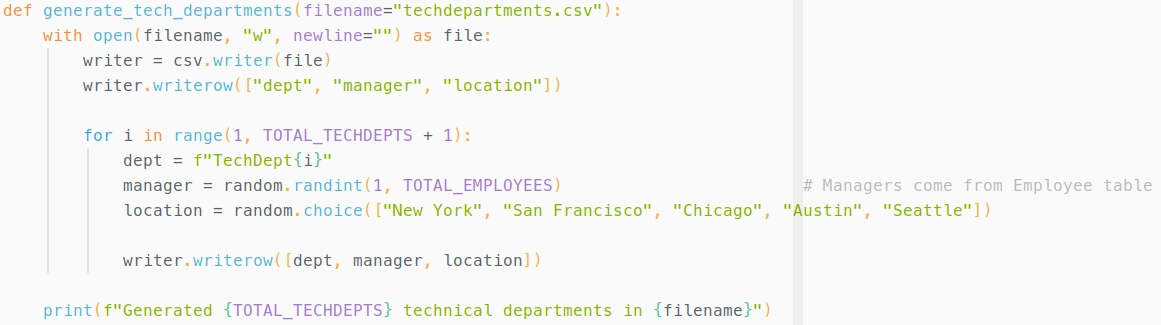
\includegraphics[width=0.8\textwidth]{Pics/TechDeptQuery.jpg}
    \caption{Script für Erstellung von TechDept}
    \label{fig:ScriptTechDept}
\end{figure}

\begin{figure}[htbp]
    \centering
    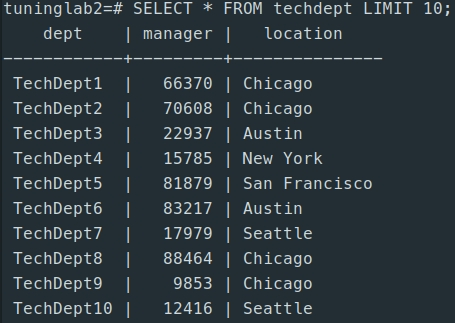
\includegraphics[width=0.8\textwidth]{Pics/TechDeptResult.jpg}
    \caption{Ergebnis TechDept}
    \label{fig:TechDeptResult}
\end{figure}

\subsubsection*{Students}

Für die Studententabelle wurden 100.000 Einträge erzeugt. Jede Person erhielt:

\begin{itemize}
    \item eine eindeutige Sozialversicherungsnummer
    \item einen eindeutigen Namen
    \item einen zufälligen Kurs und zufällige Note
\end{itemize}

\begin{figure}[htbp]
    \centering
    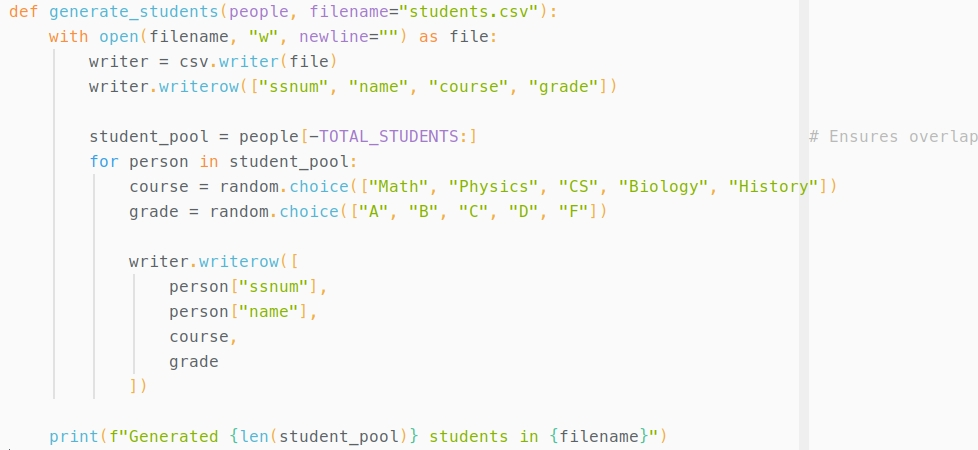
\includegraphics[width=0.8\textwidth]{Pics/StudentsScript.jpg}
    \caption{Script für Erstellung von Students}
    \label{fig:ScriptStudents}
\end{figure}

\begin{figure}[htbp]
    \centering
    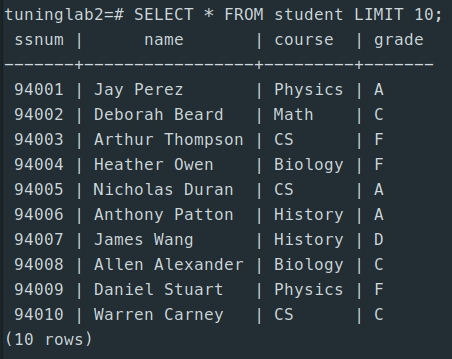
\includegraphics[width=0.8\textwidth]{Pics/StudentsResult.jpg}
    \caption{Auszug aus Students}
    \label{fig:StudentsResult}
\end{figure}

\subsubsection*{Employee}

Für die Mitarbeitertabelle wurden 100.000 Einträge erzeugt. Jede Person erhielt:

\begin{itemize}
    \item eine eindeutige Sozialversicherungsnummer
    \item einen eindeutigen Namen
    \item eine zufällige Manager-Zuweisung
    \item mit 10-prozentiger Wahrscheinlichkeit: Zugehörigkeit zu einer technischen Abteilung
    \item zufälliges Gehalt und Anzahl an "Freunden".
\end{itemize}

\begin{figure}[htbp]
    \centering
    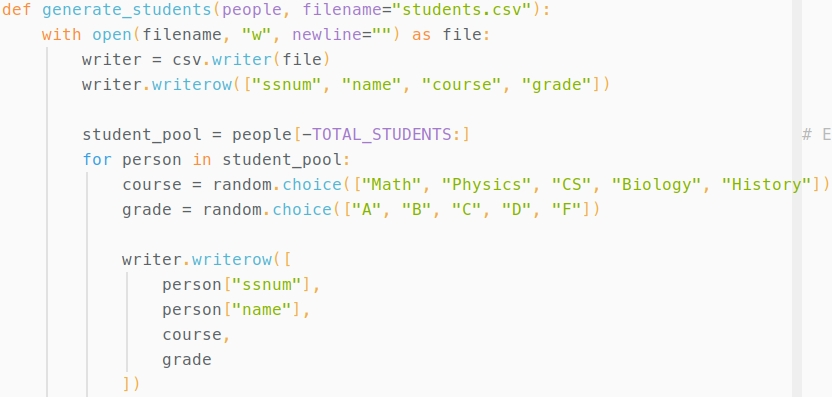
\includegraphics[width=0.8\textwidth]{Pics/ScriptEmployee.jpg}
    \caption{Script für Erstellung von Employees}
    \label{fig:ScriptEmployee}
\end{figure}

\begin{figure}[htbp]
    \centering
    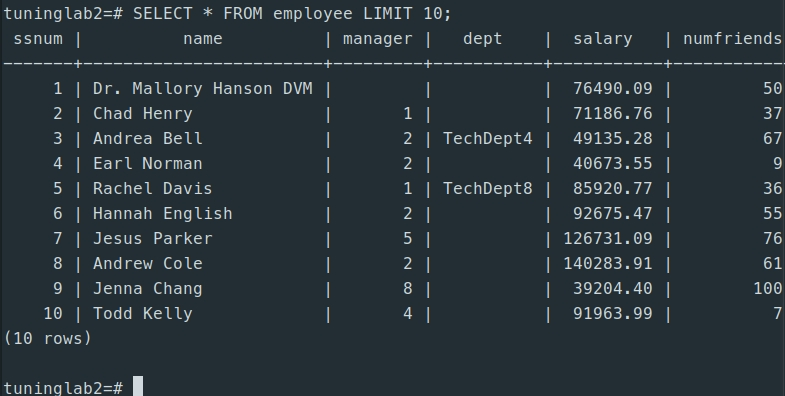
\includegraphics[width=0.8\textwidth]{Pics/EmployeeResult.jpg}
    \caption{Auszug aus Employee}
    \label{fig:EmployeeResult}
\end{figure}

\subsection*{Queries}

\subsubsection*{Query 1}

\paragraph{Original Query}

The first query shows the ssnum of all employees in tech-departments, that have a yearly salary within 1000 of the average salary over all tech-departments.

\begin{lstlisting}[style=dbtsql]
SELECT DISTINCT E1.ssnum
FROM Employee E1, Techdept T
WHERE E1.salary BETWEEN (
    (SELECT AVG(E2.salary)
     FROM Employee E2, Techdept T
     WHERE E2.dept = E1.dept
       AND E2.dept = T.dept) - 1000
) AND (
    (SELECT AVG(E2.salary)
     FROM Employee E2, Techdept T
     WHERE E2.dept = E1.dept
       AND E2.dept = T.dept) + 1000
);
\end{lstlisting}

\paragraph{Rewritten Query}

Give the rewritten query.

\begin{lstlisting}[style=dbtsql]
SELECT AVG(E.salary) as salary
FROM Employee E
JOIN Techdept T ON E.dept = T.dept;

SELECT DISTINCT E.ssnum
FROM Employee E
JOIN Techdept T ON E.dept = T.dept
WHERE E.salary BETWEEN salary - 1000 AND salary + 1000;
\end{lstlisting}

\paragraph{Evaluation of the Execution Plans}

Give the execution plan of the original query.

{\small
\parskip0pt\begin{verbatim}
Nested Loop Inner Join
	Seq Scan on employee as e1
	Filter: ((salary >= ((SubPlan 1) - '1000'::numeric)) AND (salary <= ((SubPlan 2) + '1000'::numeric)))
		Aggregate
			Nested Loop Inner Join
				Index Only Scan using idx_techdept_dept on techdept as t_1
				Index Cond: (dept = e1.dept)
				Bitmap Heap Scan on employee as e2
				Recheck Cond: (dept = e1.dept)
					Bitmap Index Scan using idx_employee_dept
					Index Cond: (dept = e1.dept)
		Aggregate
			Nested Loop Inner Join
				Index Only Scan using idx_techdept_dept on techdept as t_2
				Index Cond: (dept = e1.dept)
				Bitmap Heap Scan on employee as e2_1
				Recheck Cond: (dept = e1.dept)
					Bitmap Index Scan using idx_employee_dept
					Index Cond: (dept = e1.dept)
	Materialize
	Seq Scan on techdept as t
\end{verbatim}}

Nested Loop Inner Join: Die Tupel in Employee werden sequentiell gelesen. Dabei wird auf die Ergebnisse der beiden Sub-Queries SubPlan1 und SubPlan2 eingeschränkt. Anschließend wird das Ergebnis mit TechDept verglichen und gejoined

SubPlan1/2: Der Index in TechDept auf techdept wird verwendet, um alle Tech-Departements zu finden, die dem TechDept in Employee entsprechen. Für den Vergleich wird der Index auf techdept in Employee verwendet. Dieser Prozess wird 2x durchgeführt, da der durchschnittliche Verdienst 2x gebraucht wird.

{\small
\parskip0pt\begin{verbatim}
Aggregate
	Hash Inner Join
	Hash Cond: (e.dept = t.dept)
		Seq Scan on employee as e
		Hash
			Seq Scan on techdept as t

Nested Loop Inner Join
	Seq Scan on employee as e
	Filter: ((salary >= '89008'::numeric) AND (salary <= '91008'::numeric))
	Memoize
		Index Only Scan using idx_techdept_dept on techdept as t
		Index Cond: (dept = e.dept)
\end{verbatim}}

Aggregate: Berechnet einen Wert auf Basis aller Datensätze, hier AVG(salary), auf Basis eines Hash Joins.

Hash Inner Join: Employee wird mit TechDept gejoined. Dies Erfolgt mit einen hash join, die Werte in beiden Tabellen werden also gelesen, dann wird ein Hash-Table auf Basis von TechDept erstellt ung mit Employee verglichen.

Nested Loop Inner Join: Die Werte in Employee werden sequentiell gelesen und nur Werte mit dem entsprechenden salary ausgewählt. Diese Werte werden mit TechDept verglichen, dabei wird auch der Index auf TechDept verwendet und gespeichert, damit der Index für das gleiche Department nicht mehrmals durchlaufen werden muss.

Discuss, how the execution plan changed between the original and the rewritten query. In both the interpretation of the query plans and the discussion focus on the crucial parts, i.e., the parts of the query plans that cause major runtime differences.

In der naiven Query werden für jedes Tupel in Employee zwei Joins mit jeweils einem Aggregate ausgeführt, während nach der Optimierung der durchschnittliche Wert 1x berechnet und dann wiederverwendet wird.

\paragraph{Experiment}

\begin{table}[H]
  \centering
  \begin{tabular}{l|r}
    & Runtime [sec] \tabularnewline
    \hline
    Original query & 10.7524 seconds \tabularnewline
    Rewritten query & 0.2958 seconds \tabularnewline
  \end{tabular}
\end{table}

Die verbesserte Query ist wesentlich schneller, da in der originalen Anfrage für jedes Tupel in Employee zwei Joins und dazu jeweils ein Aggregate berechnet werden müssen, was sehr zeit- und rechenaufwändige Operationen sind. Die verbesserte Query berechnet den Wert für die Einschränkung in Employee 1x und verwendet diesen dann immer wieder weiter.

\subsubsection*{Query 2}

\paragraph{Original Query}

Give the second type of query that might be hard for your database to optimize.

\begin{lstlisting}[style=dbtsql]
SELECT ssnum
FROM Employee
WHERE dept IN (SELECT dept FROM Techdept)
\end{lstlisting}

\paragraph{Rewritten Query}

Give the rewritten query.

\begin{lstlisting}[style=dbtsql]
SELECT ssnum
FROM Employee, Techdept
WHERE Employee.dept = Techdept.dept
\end{lstlisting}

\paragraph{Evaluation of the Execution Plans}

{\small
\parskip0pt\begin{verbatim}
('Nested Loop  (cost=0.15..5212.39 rows=10007 width=4) (actual time=0.041..34.670 rows=10061 loops=1)',)
->  Seq Scan on employee  (cost=0.00..2723.00 rows=100000 width=14) (actual time=0.004..7.640 rows=100000 loops=1)',)
	->  Memoize  (cost=0.15..0.16 rows=1 width=10) (actual time=0.000..0.000 rows=0 	     loops=100000)',)
		  ->  	Index Only Scan using idx_techdept_dept on techdept  					(cost=0.14..0.15 rows=1 width=10) (actual time=0.004..0.004 rows=1 			loops=11)',)('Index Cond: (dept = employee.dept)',)
\end{verbatim}}

Nested Loop: For each employee, PostgreSQL checks if their dept exists in techdept, leading to many repeated sub-queries.

Seq Scan on employee: Scans the entire employee table row by row without using any index, which is slow for large datasets.

Memoize: Caches previous techdept lookups to avoid querying the same department multiple times, but still not optimal with many unique dept values.

Index Only Scan on techdept: Uses the index to check if the employee’s department exists, but this check is done 100,000 times.

{\small
\parskip0pt\begin{verbatim}
('Merge Join  (cost=1.56..1077.82 rows=10007 width=4) (actual time=0.070..5.647 rows=10061 loops=1)',)
 ->  Index Scan using idx_employee_dept on employee  (cost=0.29..9504.86 rows=100000 width=14) (actual time=0.028..4.032 rows=10062 loops=1)',)
	->  	Sort  (cost=1.27..1.29 rows=10 width=10) (actual time=0.040..0.042 rows=10 	      	loops=1)',)
		('        Sort Key: techdept.dept',)
		('        Sort Method: quicksort  Memory: 25kB',)
		->  	Seq Scan on techdept  (cost=0.00..1.10 rows=10 width=10) (actual 				time=0.008..0.009 rows=10 loops=1)
\end{verbatim}}

Merge Join: Combines rows from employee and techdept where the dept values match, using sorted input for efficient merging.

Index Scan on employee: Quickly retrieves employee rows by scanning the index to get sorted dept values.

Sort on Techdept: Sorts values to prepare them for the merge join.

Seq Scan on Techdept: Reads all rows from the small techdept table sequentially before sorting.

Naive Query: Does a sequential scan over all employee rows.

\begin{itemize}
\item For each row, it checks if dept is in techdept using index lookup.
\item Slower overall due to repeated subqueries.
\end{itemize}

Tuned Query: Uses Merge Join with:
\begin{itemize}
\item Index Scan on employee.dept
\item Sorted Scan on techdept
\item Optimizer uses indexes and sorting efficiently.
\item Much faster due to bulk processing and join strategy.
\end{itemize}


\paragraph{Experiment}

Give the runtimes of the original and the rewritten query.

\begin{table}[H]
  \centering
  \begin{tabular}{l|r}
    & Runtime [sec] \tabularnewline
    \hline
    Original query  & 0.1140 seconds \tabularnewline
    Rewritten query & 0.0814 seconds \tabularnewline
  \end{tabular}
\end{table}

Discuss, why the rewritten query is (or is not) faster than the original query.

In der naiven Anfrage wird für jedes Tupel in Employee eine Anfrage in TechDept ausgeführt. Die optimierte Query verwendet die vorhandenen Indizes effizient und führt die Ergebnisse bereits vorab zusammen und filtert sie.

\subsection*{Time Spent on this Assignment}

Time in hours per person: \textbf{4}

\subsection*{References}

\begin{table}[H]
  \centering
  \begin{tabular}{c}
    \hline
    \textbf{Important:} Reference your information sources! \tabularnewline
    Remove this section if you use footnotes to reference your information sources. \tabularnewline
    \hline
  \end{tabular}
\end{table}

\end{document}
